\documentclass[svgnames,11pt]{beamer}
\input{/home/tof/Documents/Cozy/latex-include/preambule_commun.tex}
\input{/home/tof/Documents/Cozy/latex-include/preambule_beamer.tex}
%\usepackage{pgfpages} \setbeameroption{show notes on second screen=left}
\author[]{Christophe Viroulaud}
\title{Représentation des entiers - exercices \\Correction}
\date{\framebox{\textbf{DonRep 03}}}
%\logo{}
\institute{Première - NSI}

\begin{document}
\begin{frame}
    \titlepage
\end{frame}
\section{Exercice 1}
\begin{frame}
    \frametitle{Exercice 1}

    \begin{center}
        \begin{tabular}{|*{2}{c|}}
            \hline
            décimal & binaire \\
            \hline
            0       & 0000    \\
            1       & 0001    \\
            2       & 0010    \\
            3       & 0011    \\
            4       & 0100    \\
            5       & 0101    \\
            6       & 0110    \\
            7       & 0111    \\
            8       & 1000    \\
            9       & 1001    \\
            10      & 1010    \\
            \hline
        \end{tabular}
    \end{center}

\end{frame}
\begin{frame}
    \frametitle{}

    \begin{center}
        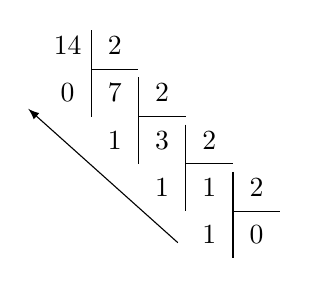
\begin{tikzpicture}
            \node at(0,0){14};
            \node at(0.6,0){2};
            \node at(0,-0.6){0};
            \node at(0.6,-0.6){7};
            \draw (0.3,0.2)--(0.3,-0.9);
            \draw (0.3,-0.3)--(0.9,-0.3);

            \node at(1.2,-0.6){2};
            \node at(0.6,-1.2){1};
            \node at(1.2,-1.2){3};
            \draw (0.9,-0.4)--(0.9,-1.5);
            \draw (0.9,-0.9)--(1.5,-0.9);

            \node at(1.8,-1.2){2};
            \node at(1.2,-1.8){1};
            \node at(1.8,-1.8){1};
            \draw (1.5,-1.0)--(1.5,-2.1);
            \draw (1.5,-1.5)--(2.1,-1.5);

            \node at(2.4,-1.8){2};
            \node at(1.8,-2.4){1};
            \node at(2.4,-2.4){0};
            \draw (2.1,-1.6)--(2.1,-2.7);
            \draw (2.1,-2.1)--(2.7,-2.1);

            \draw [->,>=latex] (1.4,-2.5) -- (-0.5,-0.8);
        \end{tikzpicture}
    \end{center}

\end{frame}
\begin{frame}
    \frametitle{}

    \begin{itemize}
        \item $14_{10} \rightarrow 00001110_2$
        \item $222_{10} \rightarrow 11011110_2$
        \item $42_{10} \rightarrow 00101010_2$
        \item $79_{10} \rightarrow 01001111_2$
    \end{itemize}

\end{frame}
\section{Exercice 2}
\begin{frame}[fragile]
    \frametitle{Exercice 2}

    \begin{center}
        \begin{lstlisting}[language=Python , basicstyle=\ttfamily\small, xleftmargin=2em, xrightmargin=2em]
n = int(input("Entrer un entier positif: "))
res = ""
while (n > 0):
    res = str(n % 2)+res
    n = n//2
print(res)
\end{lstlisting}
        \captionof{code}{Conversion décimal $\rightarrow$ binaire}
        \label{CODE}
    \end{center}

\end{frame}
\section{Exercice 3}
\begin{frame}
    \frametitle{Exercice 3}
    $$1×2^3+0×2^2+1×2^1+0×2^0 = 10$$
    \begin{itemize}
        \item $1010_2 \rightarrow 10_{10}$
        \item $111110_2 \rightarrow 62_{10}$
        \item $100101001_2 \rightarrow 297_{10}$
    \end{itemize}

\end{frame}
\section{Exercice 4}
\begin{frame}
    \frametitle{Exercice 4}
    On décompose en blocs de 4 bits:
    $$1001_2~0101_2 = 9_{16}~5_{16}$$
    \begin{itemize}
        \item $10010101_2 \rightarrow 95_{16}$
        \item $11010101_2 \rightarrow D5_{16}$
        \item $100010001_2 \rightarrow 111_{16}$
        \item $11001101001010_2 \rightarrow 334A_{16}$
    \end{itemize}

\end{frame}
\section{Exercice 5}
\begin{frame}
    \frametitle{Exercice 5}


    \begin{itemize}
        \item $AA=1010_21010_2=10101010$
        \item $BB8=1011_2 1011_2 1000_2=101110111000$
        \item $B×16^3+E×16^2+E×16^1+F×16^0=11×16^3+14×16^2+14×16^1+15×16^0=48879$
    \end{itemize}
\end{frame}
\section{Exercice 6}
\begin{frame}
    \frametitle{Exercice 6}

    \begin{itemize}
        \item $10_{10}=00001010_2\;donc\;-10_{10}=11110101+1=11110110_2$
        \item $128_{10}=10000000_2\;donc\;-128_{10}=01111111+1=10000000_2$
              \begin{aretenir}[Remarque]
                  Nous remarquons qu'il s'agit de la même représentation que 128: sur 8 bits, nous ne pouvons pas représenter l'entier positif 128!!!
              \end{aretenir}
        \item $42_{10}=00101010_2 donc -42_{10}=11010101+1=11010110_2$
        \item $97_{10}=01100001_2$
    \end{itemize}

\end{frame}
\section{Exercice 7}
\begin{frame}
    \frametitle{Exercice 7}
    Première méthode:
    \begin{itemize}
        \item  $11100111_2=231_{10}\;et\;231-2^8=-25$
        \item  $11000001_2=193_{10}\;et\;193-2^8=-63$
    \end{itemize}

\end{frame}
\begin{frame}
    \frametitle{Exercice 7}
    Deuxième méthode:
    \begin{itemize}
        \item Le complément à 2 de $11100111_2$ vaut $00011000_2$. Ensuite $00011000_2+1_2=00011001_2=25_{10}$ donc $11100111_2=-25_{10}$.
        \item Le complément à 2 de $11000001_2$ vaut $00111110_2$. Ensuite $00111110_2+1_2=00111111_2=63_{10}$ donc $11000001_2=-63_{10}$.
    \end{itemize}

\end{frame}
\section{Exercice 8}
\begin{frame}
    \frametitle{Exercice 8}
    $$39+110=00100111_2+01101110_2=10010101_2=149$$
    \begin{center}
        \begin{tabular}{*{9}{c}}
              & {\small 1}&  {\small 1} &   & {\small 1} & {\small 1} &  {\small 1} &   &    \\
              & 0 & 0 & 1 & 0 & 0 & 1 & 1 & 1 \\
            + & 0 & 1 & 1 & 0 & 1 & 1 & 1 & 0 \\
            \hline
              & 1 & 0 & 0 & 1 & 0 & 1 & 0 & 1 \\
        \end{tabular}
    \end{center}

\end{frame}
\begin{frame}

    \begin{enumerate}
        \item $39+110=00100111_2+01101110_2=10010101_2=149$ 
        \item $-53+35=11001011_2+00100011_2=11101110_2=-18 (238-256)$
        \item $119-8=01110111_2+11111000_2=01101111_2=111$ 
        \begin{aretenir}[Remarque]
            Les chiffres au-delà de 8 bits sont tronqués.
        \end{aretenir}
        \item $19-93=00010011_2+10100011_2=10110110_2=-74 (182-256)$
    \end{enumerate}

\end{frame}
\section{Exercice 9}
\begin{frame}
    \frametitle{Exercice 9}

    $$500Go=5×10^{11}o$$
    \begin{center}
        \begin{tabular}{|*{3}{c|}}
            \hline
            gibioctet (Gio)&1&?\\
            \hline
            octet (o)&1 073 741 824&$5×10^{11}$\\
            \hline
        \end{tabular}
    \end{center}
$$\frac{5×10^{11}×1}{1 073 741 824}=465$$
\begin{center}
    Le système d'exploitation affiche la capacité en Gio et non en Go.
\end{center}
\end{frame}
\end{document}